\documentclass[]{article}
\usepackage{lmodern}
\usepackage{amssymb,amsmath}
\usepackage{ifxetex,ifluatex}
\usepackage{fixltx2e} % provides \textsubscript
\ifnum 0\ifxetex 1\fi\ifluatex 1\fi=0 % if pdftex
  \usepackage[T1]{fontenc}
  \usepackage[utf8]{inputenc}
\else % if luatex or xelatex
  \ifxetex
    \usepackage{mathspec}
  \else
    \usepackage{fontspec}
  \fi
  \defaultfontfeatures{Ligatures=TeX,Scale=MatchLowercase}
\fi
% use upquote if available, for straight quotes in verbatim environments
\IfFileExists{upquote.sty}{\usepackage{upquote}}{}
% use microtype if available
\IfFileExists{microtype.sty}{%
\usepackage{microtype}
\UseMicrotypeSet[protrusion]{basicmath} % disable protrusion for tt fonts
}{}
\usepackage[margin=1in]{geometry}
\usepackage{hyperref}
\hypersetup{unicode=true,
            pdfborder={0 0 0},
            breaklinks=true}
\urlstyle{same}  % don't use monospace font for urls
\usepackage{color}
\usepackage{fancyvrb}
\newcommand{\VerbBar}{|}
\newcommand{\VERB}{\Verb[commandchars=\\\{\}]}
\DefineVerbatimEnvironment{Highlighting}{Verbatim}{commandchars=\\\{\}}
% Add ',fontsize=\small' for more characters per line
\usepackage{framed}
\definecolor{shadecolor}{RGB}{248,248,248}
\newenvironment{Shaded}{\begin{snugshade}}{\end{snugshade}}
\newcommand{\KeywordTok}[1]{\textcolor[rgb]{0.13,0.29,0.53}{\textbf{#1}}}
\newcommand{\DataTypeTok}[1]{\textcolor[rgb]{0.13,0.29,0.53}{#1}}
\newcommand{\DecValTok}[1]{\textcolor[rgb]{0.00,0.00,0.81}{#1}}
\newcommand{\BaseNTok}[1]{\textcolor[rgb]{0.00,0.00,0.81}{#1}}
\newcommand{\FloatTok}[1]{\textcolor[rgb]{0.00,0.00,0.81}{#1}}
\newcommand{\ConstantTok}[1]{\textcolor[rgb]{0.00,0.00,0.00}{#1}}
\newcommand{\CharTok}[1]{\textcolor[rgb]{0.31,0.60,0.02}{#1}}
\newcommand{\SpecialCharTok}[1]{\textcolor[rgb]{0.00,0.00,0.00}{#1}}
\newcommand{\StringTok}[1]{\textcolor[rgb]{0.31,0.60,0.02}{#1}}
\newcommand{\VerbatimStringTok}[1]{\textcolor[rgb]{0.31,0.60,0.02}{#1}}
\newcommand{\SpecialStringTok}[1]{\textcolor[rgb]{0.31,0.60,0.02}{#1}}
\newcommand{\ImportTok}[1]{#1}
\newcommand{\CommentTok}[1]{\textcolor[rgb]{0.56,0.35,0.01}{\textit{#1}}}
\newcommand{\DocumentationTok}[1]{\textcolor[rgb]{0.56,0.35,0.01}{\textbf{\textit{#1}}}}
\newcommand{\AnnotationTok}[1]{\textcolor[rgb]{0.56,0.35,0.01}{\textbf{\textit{#1}}}}
\newcommand{\CommentVarTok}[1]{\textcolor[rgb]{0.56,0.35,0.01}{\textbf{\textit{#1}}}}
\newcommand{\OtherTok}[1]{\textcolor[rgb]{0.56,0.35,0.01}{#1}}
\newcommand{\FunctionTok}[1]{\textcolor[rgb]{0.00,0.00,0.00}{#1}}
\newcommand{\VariableTok}[1]{\textcolor[rgb]{0.00,0.00,0.00}{#1}}
\newcommand{\ControlFlowTok}[1]{\textcolor[rgb]{0.13,0.29,0.53}{\textbf{#1}}}
\newcommand{\OperatorTok}[1]{\textcolor[rgb]{0.81,0.36,0.00}{\textbf{#1}}}
\newcommand{\BuiltInTok}[1]{#1}
\newcommand{\ExtensionTok}[1]{#1}
\newcommand{\PreprocessorTok}[1]{\textcolor[rgb]{0.56,0.35,0.01}{\textit{#1}}}
\newcommand{\AttributeTok}[1]{\textcolor[rgb]{0.77,0.63,0.00}{#1}}
\newcommand{\RegionMarkerTok}[1]{#1}
\newcommand{\InformationTok}[1]{\textcolor[rgb]{0.56,0.35,0.01}{\textbf{\textit{#1}}}}
\newcommand{\WarningTok}[1]{\textcolor[rgb]{0.56,0.35,0.01}{\textbf{\textit{#1}}}}
\newcommand{\AlertTok}[1]{\textcolor[rgb]{0.94,0.16,0.16}{#1}}
\newcommand{\ErrorTok}[1]{\textcolor[rgb]{0.64,0.00,0.00}{\textbf{#1}}}
\newcommand{\NormalTok}[1]{#1}
\usepackage{graphicx,grffile}
\makeatletter
\def\maxwidth{\ifdim\Gin@nat@width>\linewidth\linewidth\else\Gin@nat@width\fi}
\def\maxheight{\ifdim\Gin@nat@height>\textheight\textheight\else\Gin@nat@height\fi}
\makeatother
% Scale images if necessary, so that they will not overflow the page
% margins by default, and it is still possible to overwrite the defaults
% using explicit options in \includegraphics[width, height, ...]{}
\setkeys{Gin}{width=\maxwidth,height=\maxheight,keepaspectratio}
\IfFileExists{parskip.sty}{%
\usepackage{parskip}
}{% else
\setlength{\parindent}{0pt}
\setlength{\parskip}{6pt plus 2pt minus 1pt}
}
\setlength{\emergencystretch}{3em}  % prevent overfull lines
\providecommand{\tightlist}{%
  \setlength{\itemsep}{0pt}\setlength{\parskip}{0pt}}
\setcounter{secnumdepth}{0}
% Redefines (sub)paragraphs to behave more like sections
\ifx\paragraph\undefined\else
\let\oldparagraph\paragraph
\renewcommand{\paragraph}[1]{\oldparagraph{#1}\mbox{}}
\fi
\ifx\subparagraph\undefined\else
\let\oldsubparagraph\subparagraph
\renewcommand{\subparagraph}[1]{\oldsubparagraph{#1}\mbox{}}
\fi

%%% Use protect on footnotes to avoid problems with footnotes in titles
\let\rmarkdownfootnote\footnote%
\def\footnote{\protect\rmarkdownfootnote}

%%% Change title format to be more compact
\usepackage{titling}

% Create subtitle command for use in maketitle
\providecommand{\subtitle}[1]{
  \posttitle{
    \begin{center}\large#1\end{center}
    }
}

\setlength{\droptitle}{-2em}

  \title{}
    \pretitle{\vspace{\droptitle}}
  \posttitle{}
    \author{}
    \preauthor{}\postauthor{}
    \date{}
    \predate{}\postdate{}
  

\begin{document}

\section{Exploración de datos - Top 50 canciones
(Spotify)}\label{exploracion-de-datos---top-50-canciones-spotify}

\subsubsection{Utilizamos el dataset obtenido mediante el script
0-get-data.R}\label{utilizamos-el-dataset-obtenido-mediante-el-script-0-get-data.r}

\begin{Shaded}
\begin{Highlighting}[]
\KeywordTok{library}\NormalTok{(ggplot2)}
\KeywordTok{library}\NormalTok{(colorspace)}
\KeywordTok{library}\NormalTok{(DataExplorer)}
\KeywordTok{library}\NormalTok{(tidyverse)}
\end{Highlighting}
\end{Shaded}

\begin{verbatim}
## -- Attaching packages -------------------------------------------------- tidyverse 1.2.1 --
\end{verbatim}

\begin{verbatim}
## v tibble  2.1.1     v purrr   0.3.2
## v tidyr   0.8.3     v dplyr   0.8.1
## v readr   1.3.1     v stringr 1.4.0
## v tibble  2.1.1     v forcats 0.4.0
\end{verbatim}

\begin{verbatim}
## -- Conflicts ----------------------------------------------------- tidyverse_conflicts() --
## x dplyr::filter() masks stats::filter()
## x dplyr::lag()    masks stats::lag()
\end{verbatim}

\begin{Shaded}
\begin{Highlighting}[]
\NormalTok{data <-}\StringTok{ }\KeywordTok{read.csv}\NormalTok{(}\StringTok{'dataset_spotify.csv'}\NormalTok{)}
\KeywordTok{summary}\NormalTok{(data)}
\end{Highlighting}
\end{Shaded}

\begin{verbatim}
##        X                              cancion     popularidad    
##  Min.   :  1.0   Calma - Remix            : 17   Min.   : 16.00  
##  1st Qu.:213.8   Adan y Eva               : 16   1st Qu.: 74.00  
##  Median :426.5   Amanece                  : 15   Median : 79.00  
##  Mean   :426.5   Desconocidos             : 15   Mean   : 77.39  
##  3rd Qu.:639.2   Ella Quiere Beber - Remix: 14   3rd Qu.: 86.00  
##  Max.   :852.0   MIA (feat. Drake)        : 14   Max.   :100.00  
##                  (Other)                  :761                   
##          artista                                        artista_completo
##  Bad Bunny   : 82   Bad Bunny                                   : 53    
##  Anuel Aa    : 52   Paulo Londra                                : 37    
##  Paulo Londra: 45   Maluma                                      : 24    
##  Ozuna       : 35   Pedro Capó feat. Farruko                    : 17    
##  Karol G     : 33   Anuel Aa feat. Haze                         : 15    
##  Piso 21     : 26   Mau y Ricky feat. Manuel Turizo feat. Camilo: 15    
##  (Other)     :579   (Other)                                     :691    
##            album                        top_pais       puesto     
##  X 100PRE     : 59   El Top 50 de Uruguay   : 52   Min.   : 1.00  
##  Homerun      : 30   El Top 50 de Argentina : 50   1st Qu.:13.00  
##  Sueños       : 20   El Top 50 de Bolivia   : 50   Median :26.00  
##  Aura         : 19   El Top 50 de Chile     : 50   Mean   :25.56  
##  Calma (Remix): 17   El Top 50 de Colombia  : 50   3rd Qu.:38.00  
##  Amanece      : 15   El Top 50 de Costa Rica: 50   Max.   :52.00  
##  (Other)      :692   (Other)                :550                  
##   bailabilidad       energia        nota_musical      volumen       
##  Min.   :0.3000   Min.   :0.2640   Min.   : 0.00   Min.   :-11.420  
##  1st Qu.:0.6940   1st Qu.:0.6310   1st Qu.: 2.00   1st Qu.: -5.642  
##  Median :0.7600   Median :0.7115   Median : 6.00   Median : -4.529  
##  Mean   :0.7457   Mean   :0.6924   Mean   : 5.63   Mean   : -4.987  
##  3rd Qu.:0.8070   3rd Qu.:0.7800   3rd Qu.: 8.00   3rd Qu.: -3.674  
##  Max.   :0.9330   Max.   :0.9740   Max.   :11.00   Max.   : -1.694  
##                                                                     
##       modo           hablado          acustico        instrumental      
##  Min.   :0.0000   Min.   :0.0281   Min.   :0.00513   Min.   :0.0000000  
##  1st Qu.:0.0000   1st Qu.:0.0593   1st Qu.:0.12500   1st Qu.:0.0000000  
##  Median :1.0000   Median :0.1090   Median :0.25400   Median :0.0000000  
##  Mean   :0.5469   Mean   :0.1370   Mean   :0.27742   Mean   :0.0019318  
##  3rd Qu.:1.0000   3rd Qu.:0.1895   3rd Qu.:0.38300   3rd Qu.:0.0000346  
##  Max.   :1.0000   Max.   :0.5000   Max.   :0.94000   Max.   :0.3120000  
##                                                                         
##     en_vivo        positividad         tempo           duracion     
##  Min.   :0.0161   Min.   :0.1170   Min.   : 70.14   Min.   :113013  
##  1st Qu.:0.0869   1st Qu.:0.5042   1st Qu.: 94.19   1st Qu.:188746  
##  Median :0.1075   Median :0.6635   Median :103.47   Median :210774  
##  Mean   :0.1456   Mean   :0.6166   Mean   :122.69   Mean   :218461  
##  3rd Qu.:0.1580   3rd Qu.:0.7610   3rd Qu.:160.01   3rd Qu.:236174  
##  Max.   :0.8920   Max.   :0.9630   Max.   :203.93   Max.   :456940  
##                                                                     
##  tiempo_compas          fecha    
##  Min.   :3.000   2018-12-23: 59  
##  1st Qu.:4.000   2018-12-14: 36  
##  Median :4.000   2019-05-10: 31  
##  Mean   :3.992   2019-05-23: 30  
##  3rd Qu.:4.000   2019-05-17: 29  
##  Max.   :5.000   2019-05-03: 27  
##                  (Other)   :640
\end{verbatim}

\subsection{Chequeamos valores
faltantes}\label{chequeamos-valores-faltantes}

\begin{Shaded}
\begin{Highlighting}[]
\KeywordTok{sum}\NormalTok{(}\KeywordTok{is.na}\NormalTok{(data))}
\end{Highlighting}
\end{Shaded}

\begin{verbatim}
## [1] 0
\end{verbatim}

\subsection{\texorpdfstring{Analizamos \emph{popularidad} respecto de
\emph{bailabilidad} en
Argentina}{Analizamos popularidad respecto de bailabilidad en Argentina}}\label{analizamos-popularidad-respecto-de-bailabilidad-en-argentina}

\begin{Shaded}
\begin{Highlighting}[]
\KeywordTok{ggplot}\NormalTok{(}\DataTypeTok{data =} \KeywordTok{subset}\NormalTok{(data, }\DataTypeTok{top_pais=}\StringTok{'El Top 50 de Argentina'}\NormalTok{)) }\OperatorTok{+}
\StringTok{  }\KeywordTok{geom_point}\NormalTok{(}\DataTypeTok{mapping =} \KeywordTok{aes}\NormalTok{(}\DataTypeTok{x=}\NormalTok{bailabilidad, }\DataTypeTok{y=}\NormalTok{popularidad))}
\end{Highlighting}
\end{Shaded}

\includegraphics{EDA_files/figure-latex/unnamed-chunk-3-1.pdf}

\textbf{Conclusión}: Observamos que generalmente las canciones populares
son bailables, aunque existen outliers que no cumplen esto.

\begin{center}\rule{0.5\linewidth}{\linethickness}\end{center}

\subsubsection{Variedad y uso de las tonalidades: ¿Cuáles son las más
utilizadas?}\label{variedad-y-uso-de-las-tonalidades-cuales-son-las-mas-utilizadas}

\begin{Shaded}
\begin{Highlighting}[]
\KeywordTok{ggplot}\NormalTok{(}\DataTypeTok{data =}\NormalTok{ data) }\OperatorTok{+}
\StringTok{  }\KeywordTok{geom_bar}\NormalTok{(}\DataTypeTok{mapping =} \KeywordTok{aes}\NormalTok{(}\DataTypeTok{x =}\NormalTok{ nota_musical))}
\end{Highlighting}
\end{Shaded}

\includegraphics{EDA_files/figure-latex/unnamed-chunk-4-1.pdf}

\textbf{Conclusión}: según la API (y para sorpresa mía) existe una
variada utilización de las tonalidades (salvo por Re\#/Mib que
aparentemente es la menos popular)

\begin{center}\rule{0.5\linewidth}{\linethickness}\end{center}

\subsubsection{Correlación. ¿Cuál es la clave del
éxito?}\label{correlacion.-cual-es-la-clave-del-exito}

Analizaremos la correlación entre las features.

\begin{Shaded}
\begin{Highlighting}[]
\KeywordTok{plot_correlation}\NormalTok{(data, }\DataTypeTok{type=}\StringTok{"c"}\NormalTok{)}
\end{Highlighting}
\end{Shaded}

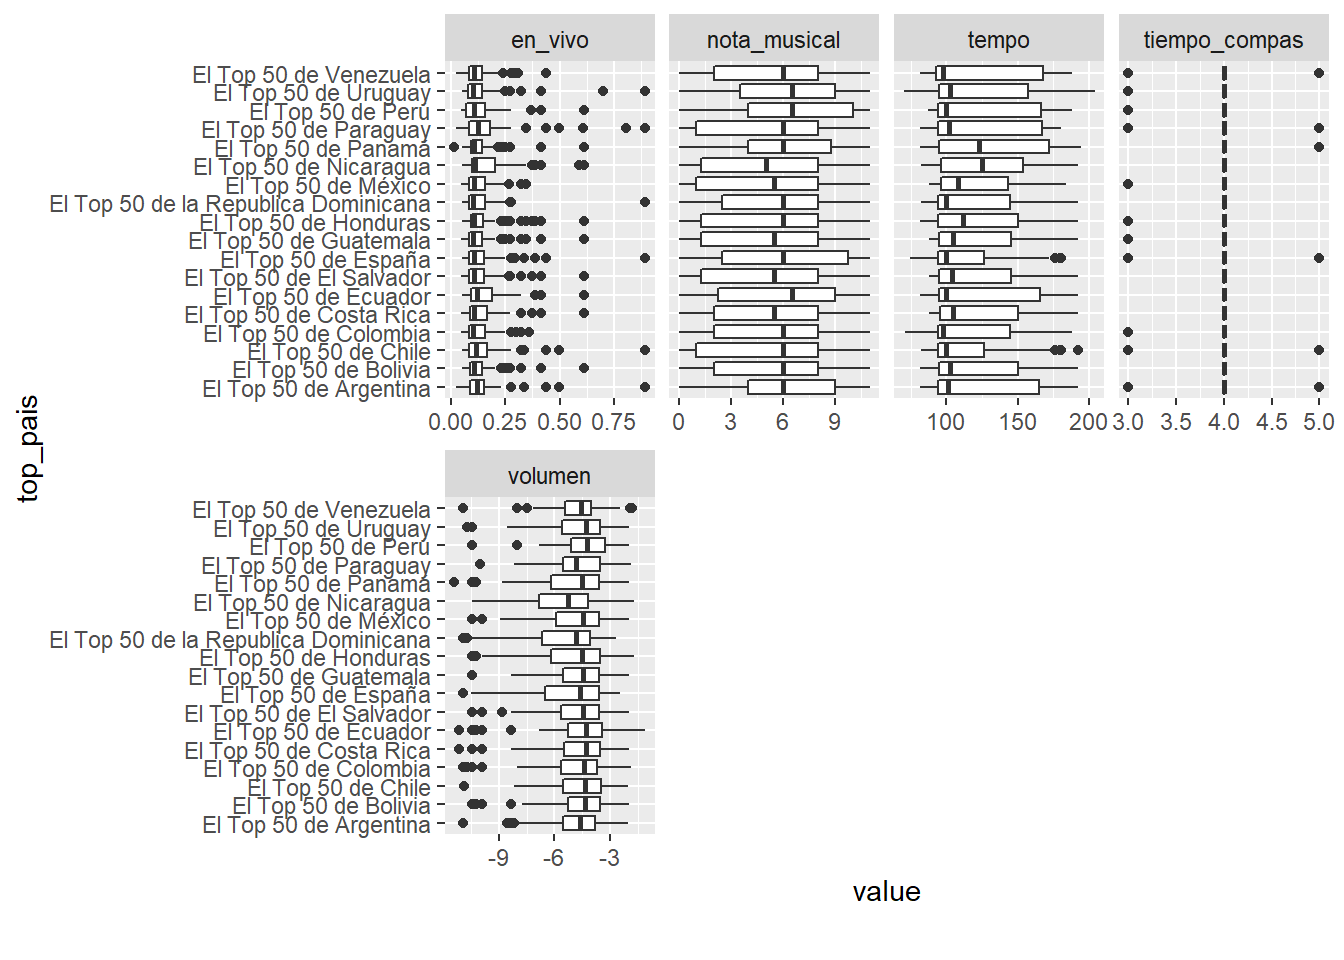
\includegraphics{EDA_files/figure-latex/unnamed-chunk-5-1.pdf}

\textbf{Conclusiones}: no observamos valores altos de correlación salvo
entre \emph{volumen} y \emph{energía}. Otras features aparentemente
relacionadas son \emph{positividad} con \emph{energía} y \emph{volumen},
\emph{tempo} con \emph{hablado}, y \emph{popularidad} con
\emph{bailabilidad} (algo que aproximadamente se mostró en el scatter
plot anterior). Resulta interesante que ninguna feature presenta
correlación alta con \emph{popularidad} o \emph{puesto}. Aparentemente
no existe la clave del éxito.

\begin{center}\rule{0.5\linewidth}{\linethickness}\end{center}

\subsubsection{Clustering}\label{clustering}

Se utilizará clustering para agrupar canciones con características
similares.

\paragraph{k-means}\label{k-means}

\begin{Shaded}
\begin{Highlighting}[]
\NormalTok{features <-}\StringTok{ }\NormalTok{data }\OperatorTok
\StringTok{  }\KeywordTok{select}\NormalTok{(bailabilidad, energia, volumen, hablado, positividad, acustico)}

\NormalTok{ncluster <-}\StringTok{ }\DecValTok{4}
\NormalTok{km <-}\StringTok{ }\KeywordTok{kmeans}\NormalTok{(features, ncluster)}
\CommentTok{# cluster <- NA }
\CommentTok{# for (n in 1:ncluster)\{}
\CommentTok{#   cluster[n] <- data[km$cluster[] == n, 'cancion']}
\CommentTok{# \}}

\NormalTok{cluster_col <-}\StringTok{ }\KeywordTok{rainbow_hcl}\NormalTok{(}\DecValTok{4}\NormalTok{)[km}\OperatorTok{$}\NormalTok{cluster]}

\CommentTok{# Plot }
\KeywordTok{pairs}\NormalTok{(features, }
      \DataTypeTok{col =}\NormalTok{ cluster_col,}
      \DataTypeTok{lower.panel =} \OtherTok{NULL}\NormalTok{,}
      \DataTypeTok{cex.labels=}\DecValTok{1}\NormalTok{, }\DataTypeTok{pch=}\DecValTok{19}\NormalTok{, }\DataTypeTok{cex =} \FloatTok{1.2}\NormalTok{)}
\end{Highlighting}
\end{Shaded}

\includegraphics{EDA_files/figure-latex/unnamed-chunk-6-1.pdf}

\subsection{Conclusiones}\label{conclusiones}

En este laboratorio se utilizaron técnicas de exploración de los datos,
con las cuales se observó la relación entre ellos y se aplicó el
algoritmo de clustering \emph{kmeans} para obtener posibles agrupaciones
de los mismos.


\end{document}
